
\section{Fundamentação Teórica}
\subsection{O Interferômetro de Michelson}

	Em 1801, o físico e médico inglês Thomas Young desenvolveu o experimento de fenda dupla que demonstrou o fenômeno de interferência luminosa. Aproximadamente 80 anos depois, o físico Albert Abraham Michelson desenvolveu um interferômetro com mecanismo similar ao de Young. Vale ressaltar que o experimento foi concebido inicialmente com o intuito de comprovar a existência o éter como meio material.
	O interferômetro de Michelson se tornou mundialmente famoso devido à sua relatividade simplicidade e alta aplicabilidade, tanto no meio didático quanto no experimental. A Figura \ref{im:int} demonstra o funcionamento do aparato.

 \begin{figure}[!htb]
 	\centering
 		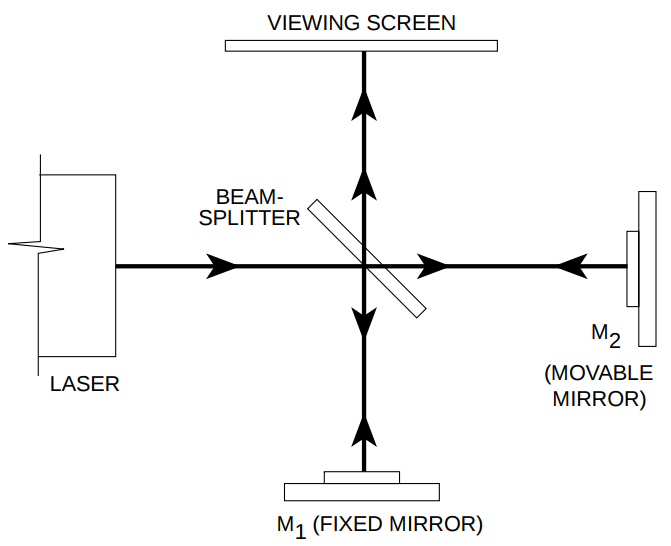
\includegraphics[scale= 0.5]{interferometro.png}
 	\caption{Interferômetro de Michelson}
 	\label{im:int}
 \end{figure}


Ao sair do laser a luz atinge o {\it beam-splitter}, onde é dividida de modo que 50\% da mesma atinja o espelho físico M1 e os outros 50\% o espelho M2. Ao atingir ambos os espelhos, a luz é refletida em direção ao {\it beam-splitter} mais uma vez. No caminho de volta, os dois feixes são projetados na tela de visualização. A separação e posteriormente união dos feixes gera uma pequena defasagem entre os mesmos, essa defasagem é o que causa a interferência. Como a diferença de fase é da ordem do comprimento de onda, faz-se necessário o uso de uma lente divergente que amplia a imagem projetada, o que possibilita a visualização do padrão de interferência.
\begin{figure}[!htb]
	\centering
		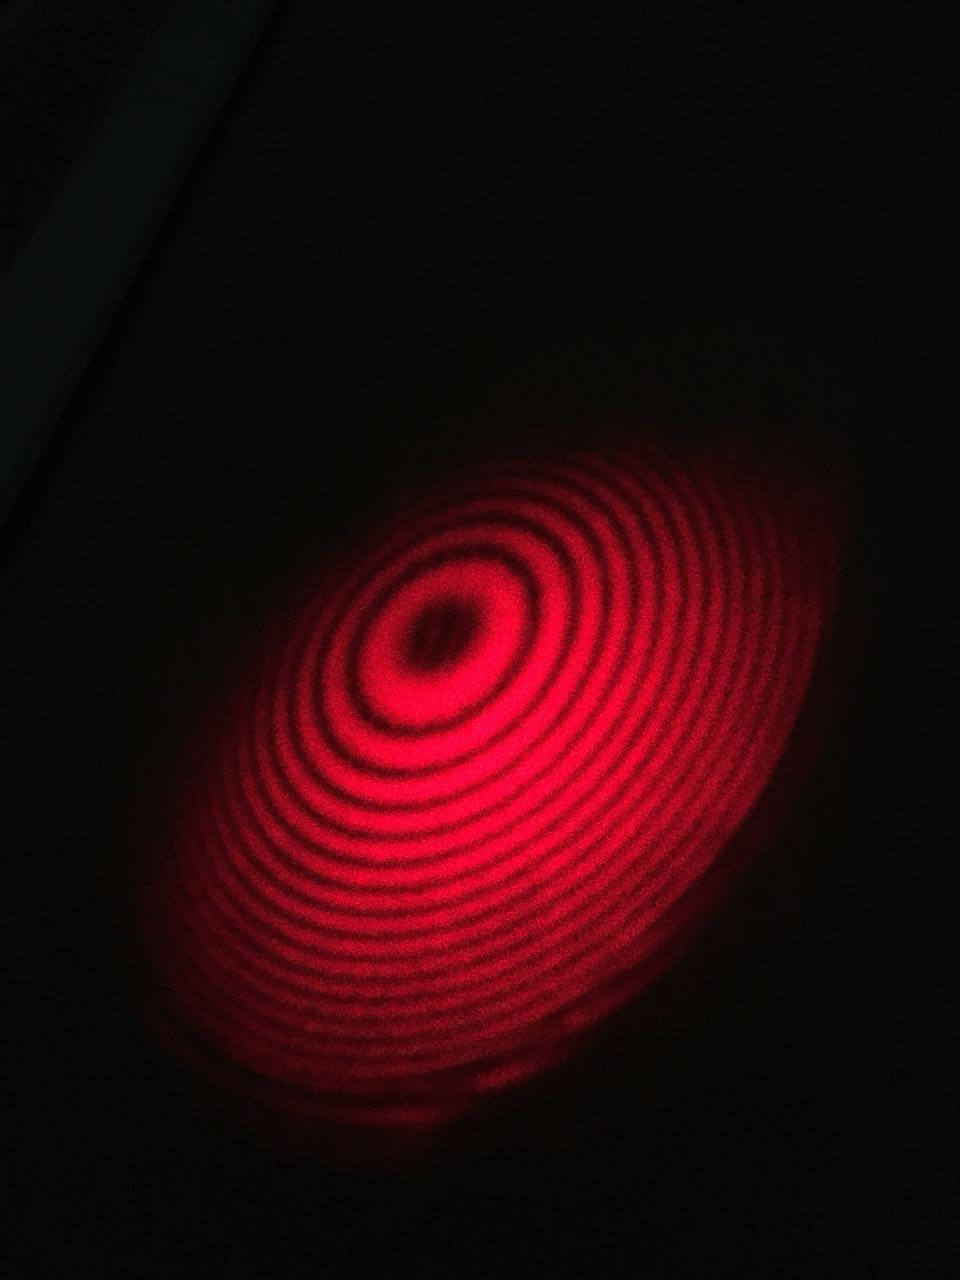
\includegraphics[scale= 0.1]{padrao.jpeg}
	\caption{Padrão de interferência}
	\label{im:pad}
\end{figure}

	A defasagem entre os feixes de luz decorre da alavanca acoplada no espelho M2, ao variar a posição da alavanca é possível gerar uma diferença de fase entre os feixes de luz no momento em que se encontram projetados.
	Ao realizar sucessivas variações na posição do espelho M2 é possível determinar o comprimento $\lambda$ a partir da distância $d_{m}$ medida ao girar a alavanca de M2 e do número de franjas de interferência usando a equação:

$\lambda =  \frac{d_{m}}{m}$

	Se $\lambda$ for conhecido, a mesma equação pode ser utilizada para determinar a distância $d_{m}$.

\subsection{Medição do índice de Refração do Ar}

	Por ser um equipamento extremamente sensível, verifica-se que vibrações como andar próximo ao aparato é o suficiente para provocar variações no padrão de interferência observado. Tendo em vista essa sensibilidade, torna-se possível medir o índice de refração do ar usando o mesmo equipamento.

	Ao posicionar uma câmara de vácuo em um dos braços do caminho óptico e variar a pressão dentro da mesma, verifica-se uma série de variações no padrão de interferência projetado.

	Considerando a pressão inicial da câmara como $P_{i}$ e a final como $P_{f}$, tem-se as equações:
\begin{equation}
\lambda_{i} = \frac{2d_{i}}{\Delta m_{i}}
\label{eq:lbd}
\end{equation}
\begin{equation}
\lambda_{f} = \frac{2d_{f}}{\Delta m_{i}}
\end{equation}
	Intuitivamente, observa-se que para a diferença de pressão $P_{f}-P_{i}$ surge a relação
\begin{equation}
\Delta m = \Delta m_{f} - \Delta m_{i}
\end{equation}
\begin{equation}
\Delta m = \frac{2d}{\lambda_{f}} - \frac{2d}{\lambda_{i}}
\end{equation}
\begin{equation}
\Delta m = \frac{2d}{\frac{\lambda_{0}}{n_{f}}} - \frac{2d}{\frac{\lambda_{0}}{n_{i}}}
\end{equation}
\begin{equation}
\Delta m = \frac{2d}{\lambda_{0}}(n_{f}-n{i})
(n_{f}-n_{i}) = \frac{\Delta m \lambda_{0}}{2d}
\end{equation}
	Dividindo a equação por $(P_{f}-P_{i})$,
\begin{equation}
\frac{n_{f}-n_{i}}{P_{f}-P_{i}} = \frac{\Delta m \lambda_{0}}{2d} \frac{1}{P_{f}-P_{i}}
\end{equation}
	De onde é possível escrever, por fim,
\begin{equation}
n_{f} = n_{i} + \frac{\Delta m \lambda}{2d \Delta P} (P_{atm}-P_{0})
\label{eq:ni}
\end{equation}
	Onde
\begin{itemize}
\item $n_{f}$: índice de refração final;
\item $n_{i}$: índice de refração inicial (vácuo);
\item $\Delta m$: variação do número de franjas;
\item $\lambda$: comprimento de onda do laser utilizado;
\item $d$: comprimento da câmara de vácuo;
\item $\Delta P$: variação de pressão registrada no manômetro;
\item $P_{atm}$: pressão atmosférica;
\item $P_{0}$: pressão inicial na câmara ($P_{0} = 0$).
\end{itemize}



